\documentclass[serif,mathserif,10pt]{beamer}
\usepackage{amsmath, amsfonts, epsfig, xspace}
\usepackage{algorithm,algorithmic}
\usepackage{pstricks,pst-node}
\usepackage{multimedia}
\usepackage[normal,tight,center]{subfigure}
\setlength{\subfigcapskip}{-.5em}
\usepackage{beamerthemesplit}
\usetheme{lankton-keynote}

\usepackage{mdframed}

\usepackage{setspace}% http://ctan.org/pkg/setspace
\let\oldframetitle\frametitle% Store \frametitle in \oldframetitle
\renewcommand{\frametitle}[1]{%
      \oldframetitle{#1}\setstretch{1.2}}

\hypersetup{colorlinks}

\newcommand{\matr}[1]{\mathbf{#1}}
\newcommand{\tran}[1]{#1^{\top}}

\def\gw#1{gravitational wave#1 (GW#1)\gdef\gw{GW}}
\def\ns#1{neutron star#1 (NS#1)\gdef\ns{NS}}

%\titlegraphic{
\includegraphics[width=0.5\textwidth]{figures/cra.png}}

\begin{document}
\setbeamertemplate{caption}{\raggedright\insertcaption\par}

\title[BNS Bursts]{Searching For Gravitational Wave Bursts From
Binary Neutron Star Coalescence}
\author{James A. Clark}
\institute{Georgia Institute of Technology}
\date{} 

%\maketitle

\begin{frame}[plain]
\titlepage
\end{frame}

\begin{frame}
    \frametitle{This Talk}
    \tableofcontents
\end{frame} 

\section{GW Bursts From BNS Mergers}

\begin{frame}
    \frametitle{Burst Signals: Short}
\end{frame}

\begin{frame}
    \frametitle{Burst Signals: Short}
    \begin{figure}
        \centering
        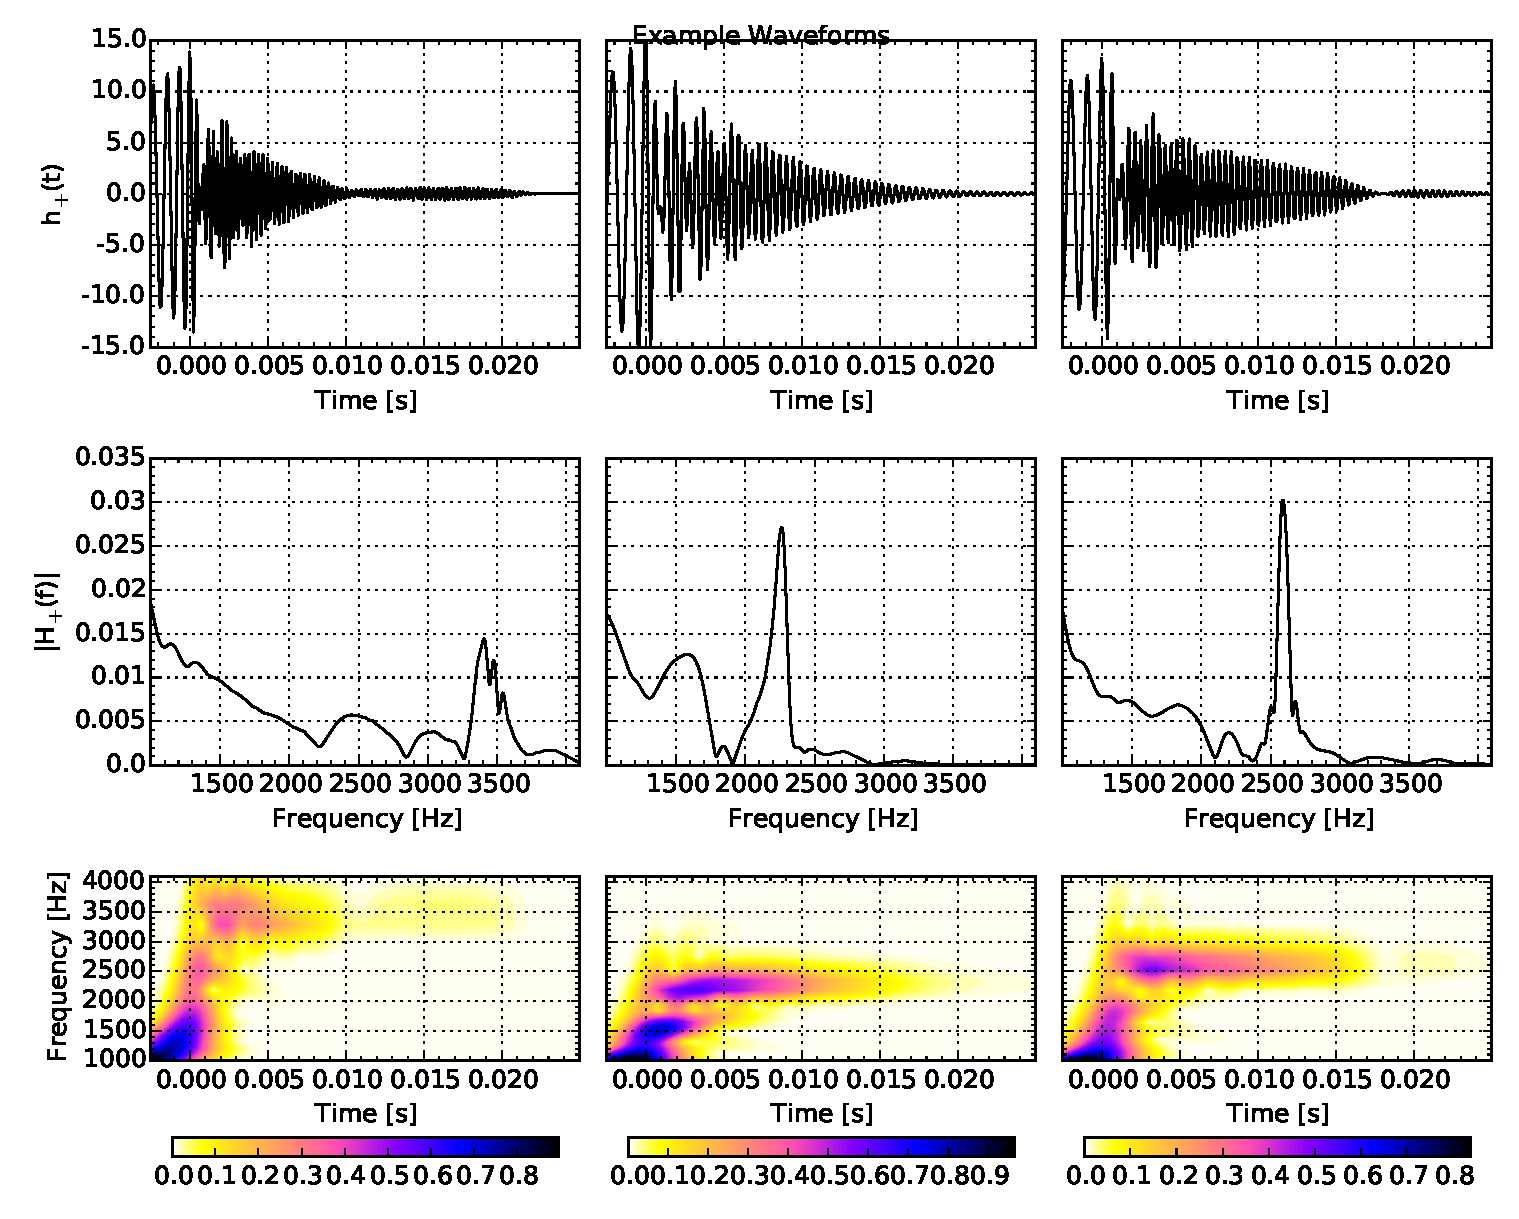
\includegraphics[width=0.9\columnwidth]{figures/example_waves.pdf}
    \end{figure}
\end{frame}

\section{GW Burst Data Analysis}

\begin{frame}
    \frametitle{GW Burst Search: Coherent WaveBurst (CWB)}
    \begin{itemize}
        \item Search for excess power in time-frequency plane
        \item Decompose data with multi-resolution wavelet basis
        \item Coherent analysis maximises likelihood over waveform \&
            sky-location
        \item Identifies statistically significant coherent power (detection),
            reconstructs GW signal
    \end{itemize}

    \begin{columns}

        \column{0.6\textwidth}

        \begin{center}
            \vspace{-0.1cm}
            \begin{figure}
                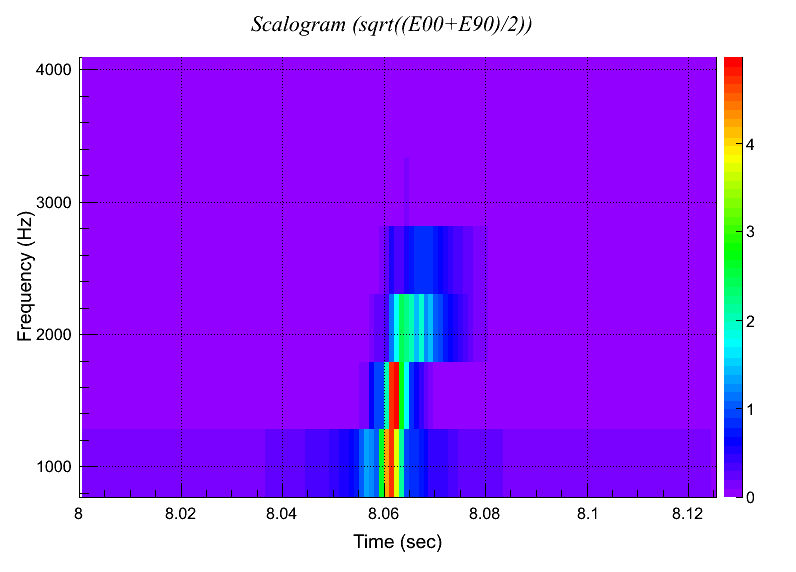
\includegraphics[width=0.7\columnwidth]{figures/L1_wf_white_inj_tf.png}
                \caption{Simulated signal}
            \end{figure}
        \end{center}

        \column{0.6\textwidth}

        \begin{center}
            \vspace{-0.1cm}
            \begin{figure}
                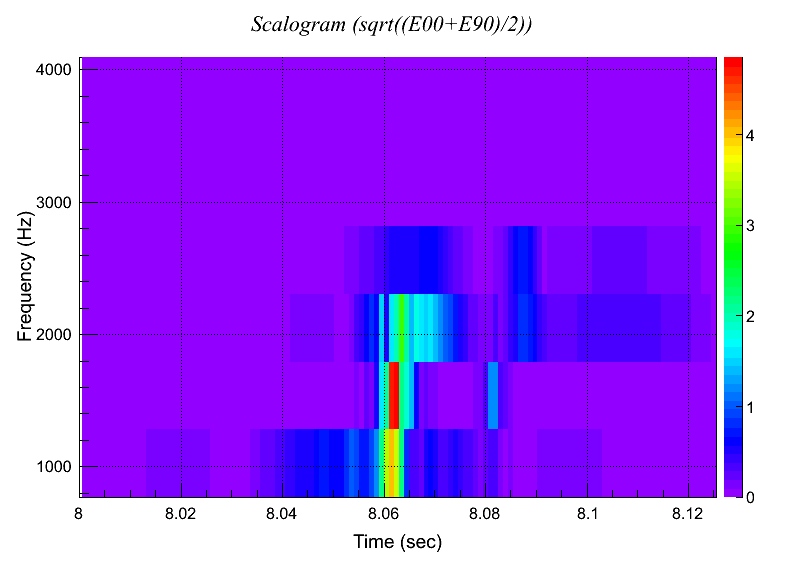
\includegraphics[width=0.7\columnwidth]{figures/L1_wf_white_rec_tf.png}
                \caption{Reconstructed signal}
            \end{figure}
        \end{center}

    \end{columns}

\end{frame}

\begin{frame}
    \frametitle{Previous Burst Detectability Study}
    \begin{quote}
        "Prospects For High Frequency Burst Searches Following Binary Neutron
        Star Coalescence With Advanced Gravitational Wave Detectors"
    \end{quote}

    Monte-Carlo analysis of burst detectability and basic parameter estimation
    of post-merger bursts
    \begin{itemize}
        \item Family of numerical waveforms with various EoS
        \item Initial detector era noise recoloured to ~2022 sensitivities
        \item Deployed CWB to detect \& reconstruct signals
        \item Compared sensitivity with optimal matched filter expectation
        \item Very simple model selection procedure for spectral analysis of
            reconstructed signals (identify post-merger scenario, measure
            dominant frequency)
    \end{itemize}

    

\end{frame}


\begin{frame}
    \frametitle{Detectability \& Frequency Recovery}

    \begin{columns}[]

        \column{0.6\textwidth}

        \begin{center}
            \vspace{-0.5cm}
            \begin{figure}
                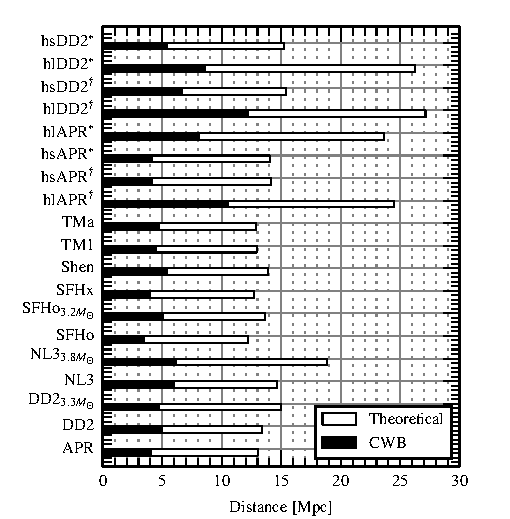
\includegraphics[width=\columnwidth]{figures/distances.pdf}
            \end{figure}
        \end{center}

        \column{0.6\textwidth}

        \begin{center}
            \vspace{-0.5cm}
            \begin{figure}
                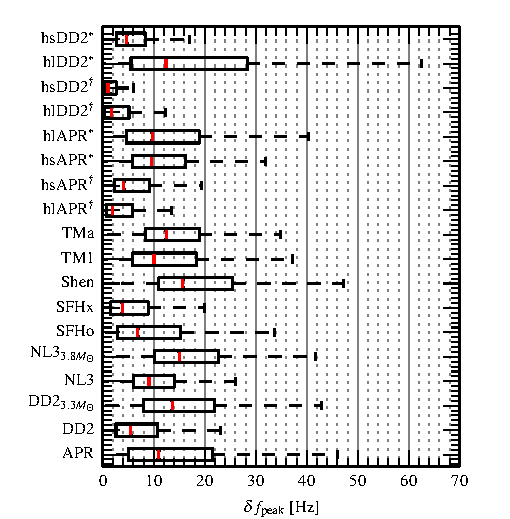
\includegraphics[width=\columnwidth]{figures/deltaFpeak.pdf}
            \end{figure}
        \end{center}

    \end{columns}

\end{frame}

\section{GW Burst Data Analysis: Future Prospects \& Development}

\begin{frame}
    \frametitle{New Study: Prospects for\dots: Round 2}
    Motivation to repeat study:
    \begin{itemize}
        \item Recent upgrades to flagship burst analysis algorithm \footnote{e.g.,
            multi-resolution analysis}
        \item Availability of more post-merger waveforms from University of Trento (also
            home of various CWB experts)
        \item Also recent development \& availability of `unmodelled' Bayesian
            analysis algorithm
        \item Tune the post-merger analysis for next year's BNS inspiral detection!
    \end{itemize}

    Participants: 

\end{frame}

\begin{frame}
    \frametitle{Enhancements \& Bayesian Methods}
\end{frame}

\begin{frame}
    \frametitle{Principal Component Analysis Of Short Bursts}

    \begin{small}
    \begin{enumerate}
        \item Organise $N$ waveforms, each containing $M$ samples, from
            numerical simulations of binary neutron star mergers into an $M\times N$
            data matrix, $\matr{X}$
        \item Align dominant features (see below), and center the data (subtract the
            mean waveform, $\matr{h}$) to get centered data matrix
            \begin{equation}
            \matr{Y}=\matr{X}-\matr{h}
        \end{equation}
        \item Find the eigenvectors $\matr{W}$ of the covariance matrix
            \begin{equation}
            \matr{C} = \tran{\matr{Y}}\matr{Y},
        \end{equation}
    \item Using $\matr{W}$, we can find the principal component
            decomposition of $\matr{X}$,
            \begin{equation}\label{eq:pca}
                \matr{Z} = \matr{X} \matr{W},
            \end{equation}
            where $\matr{W}$ has been sorted in order of descending eigenvalues, and
            $\matr{Z}$ is the \emph{score matrix}, first $p<N$ columns of
            which represent our reduced basis\footnote{One takes care, of course, to
            add the mean waveform $\matr{h}$ back on to the waveform reconstructed
        from $\matr{Z}$}.
        \item Implemented via singular value decomposition, $\matr{X} =
            \matr{U}\matr{\Sigma}\tran{\matr{W}}$ so that,
            \begin{equation}
                \matr{Z} = \matr{X} \matr{W} =
                \matr{U}\matr{\Sigma}\matr{W}\tran{\matr{W}} = \matr{U}\matr{\Sigma}
            \end{equation}
    \end{enumerate}
\end{small}
\end{frame}


\begin{frame}
    \frametitle{Short Burst PCA}

    OVERLAY PLOT WITH 3 EXAMPLE SPECTRA ON LEFT, 3 EXAMPLES ALIGNED ON RIGHT

    \begin{figure}
        \centering
        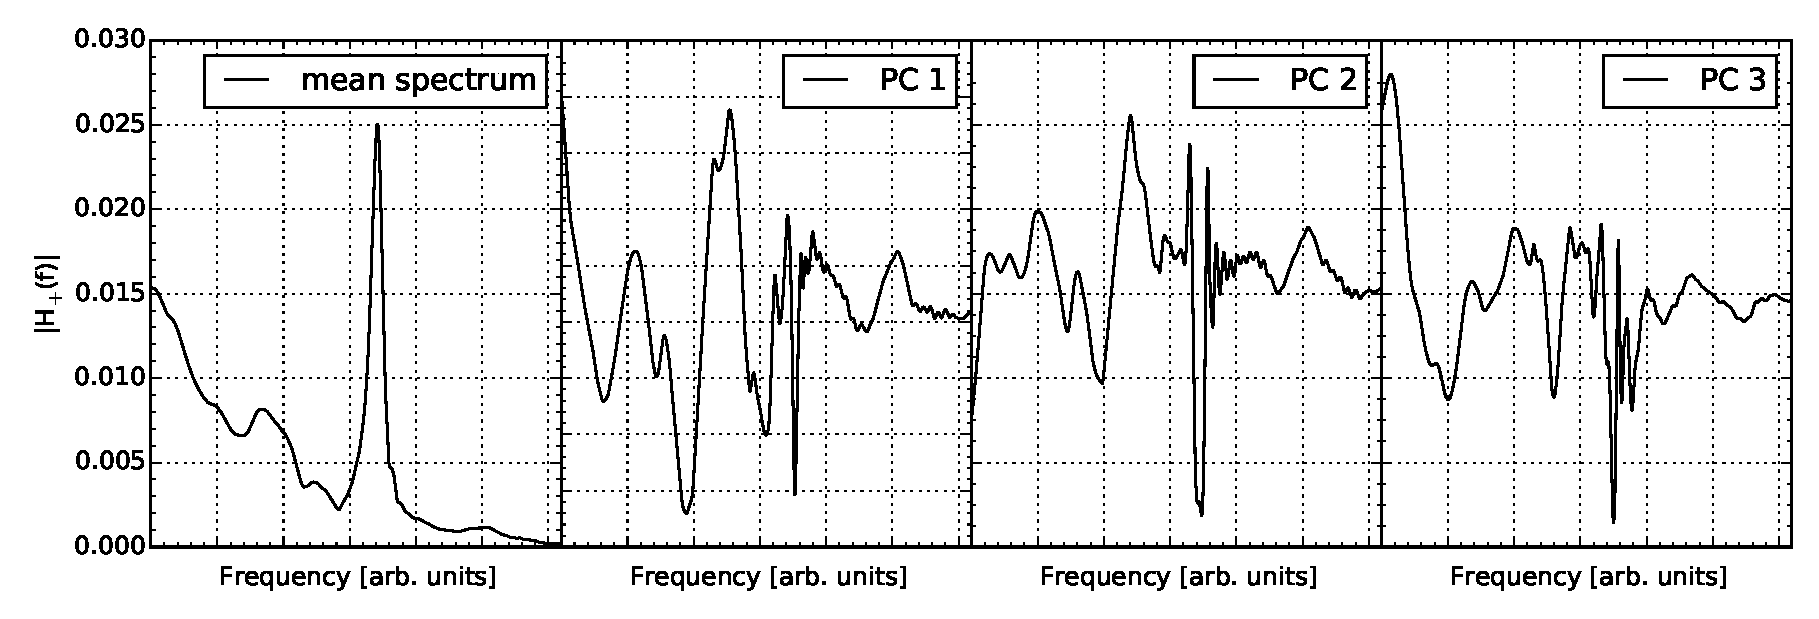
\includegraphics[width=\columnwidth]{figures/magnitude_pcs.pdf}
    \end{figure}

\end{frame}

\begin{frame}
    \frametitle{Prospects for PCA Of Short Bursts}

    \begin{columns}[]

        \column{0.5\textwidth}

        \begin{center}
            \vspace{-0.5cm}
            \begin{figure}
                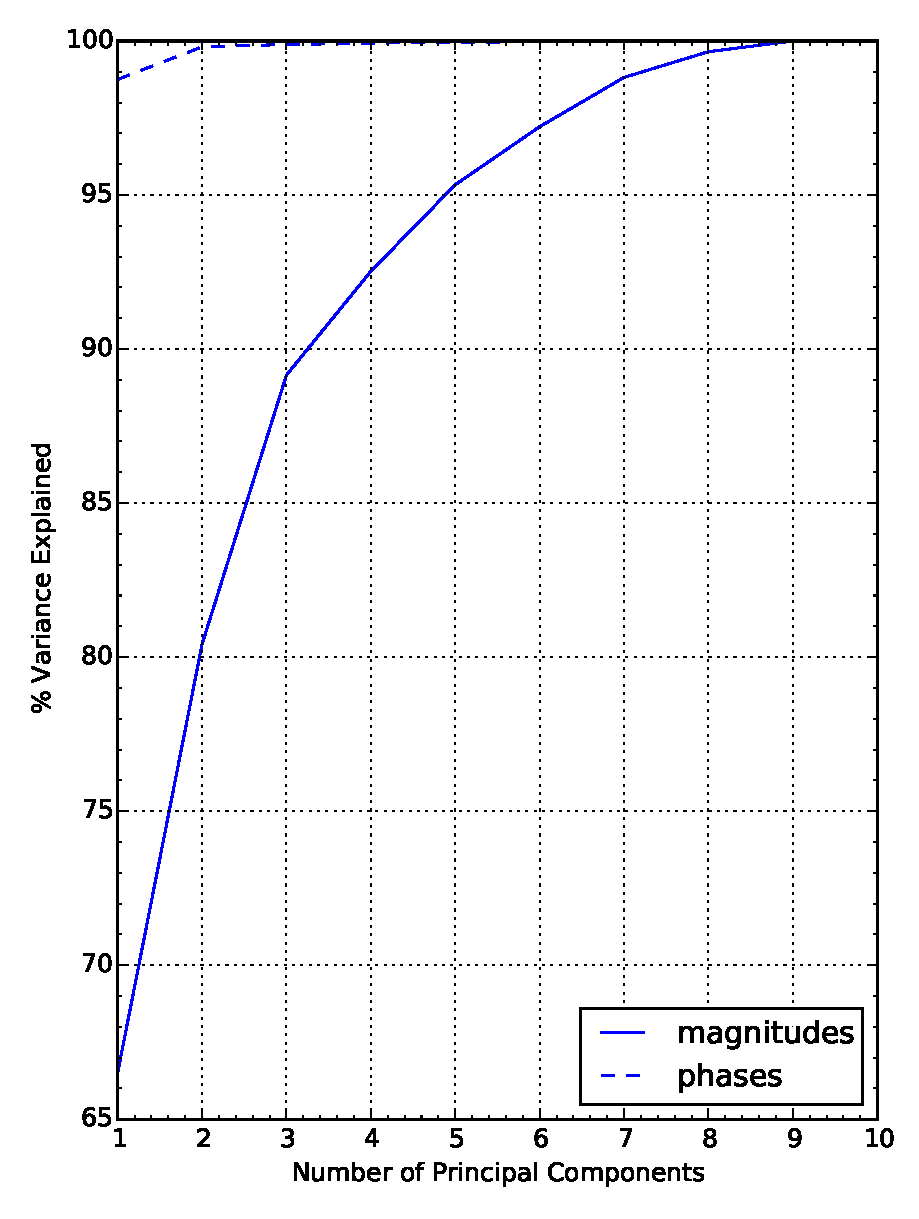
\includegraphics[width=\columnwidth]{figures/explained_variance.pdf}
            \end{figure}
        \end{center}

        \column{0.5\textwidth}

        \begin{center}
            \vspace{-0.5cm}
            \begin{figure}
                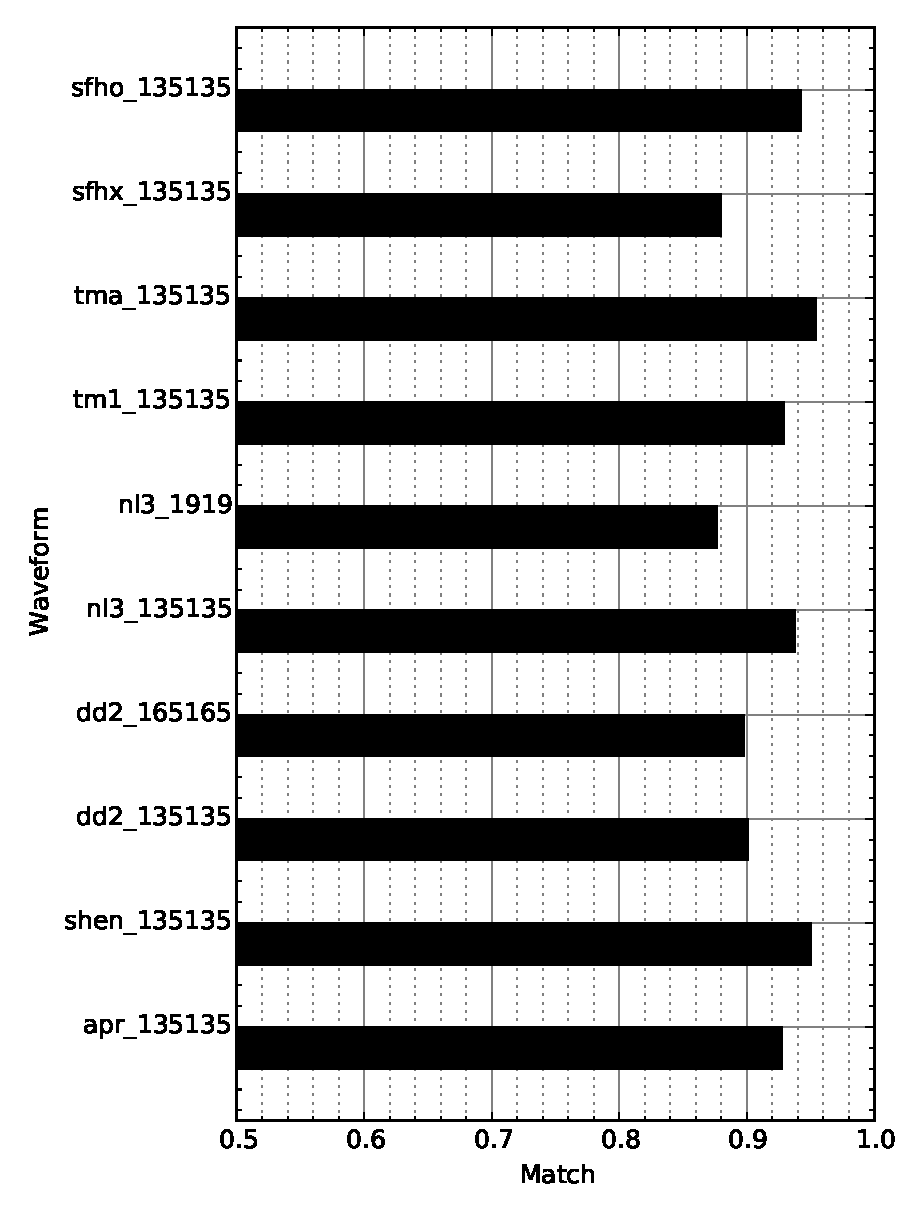
\includegraphics[width=\columnwidth]{figures/match_bars_exctestwav.pdf}
            \end{figure}
        \end{center}


    \end{columns}

\end{frame}

\begin{frame}
    \frametitle{Next Steps With PCA}

    PCA provides an (approximate) template:
    \begin{equation}
        H(f) \approx A_{\rm PCA}(f) \exp [i \phi_{\rm PCA}(f)],
    \end{equation}
    where,
    \begin{eqnarray}
        A_{\rm PCA}(f) = \sum_{i=1}^N \beta_i^{(A)}u_i^{(A)} \\ \nonumber
        \phi_{\rm PCA}(f) = \sum_{i=1}^N \beta_i^{(\phi)}u_i^{(\phi)} 
    \end{eqnarray}

    \begin{itemize}
        \item Intrinsic parameters: peak frequency (used for feature alignment)
            \& projection coefficients $\{\beta^{(A)}, \beta^{(\phi)}\}$
        \item Yield approximate waveform reconstruction \\
        \item Recover dominant \& sub-dominant frequencies \\
    \end{itemize}

    Implementation in LSC Bayesian inference package coming soon \dots

\end{frame}

\section{Other Prospects}

\begin{frame}
    \frametitle{Burst Signals: Long}
\end{frame}


\begin{frame}
    \frametitle{Searching For Long Bursts}
\end{frame}

\section{Summary \& Outlook}
\begin{frame}
    \frametitle{Summary}
\end{frame}

\appendix
\section{GW Burst Data Analysis: Future Prospects \& Development}

\begin{frame}
    \frametitle{Principal Component Analysis Of Short Bursts}



        \begin{center}
            \vspace{-0.5cm}
            \begin{figure}
                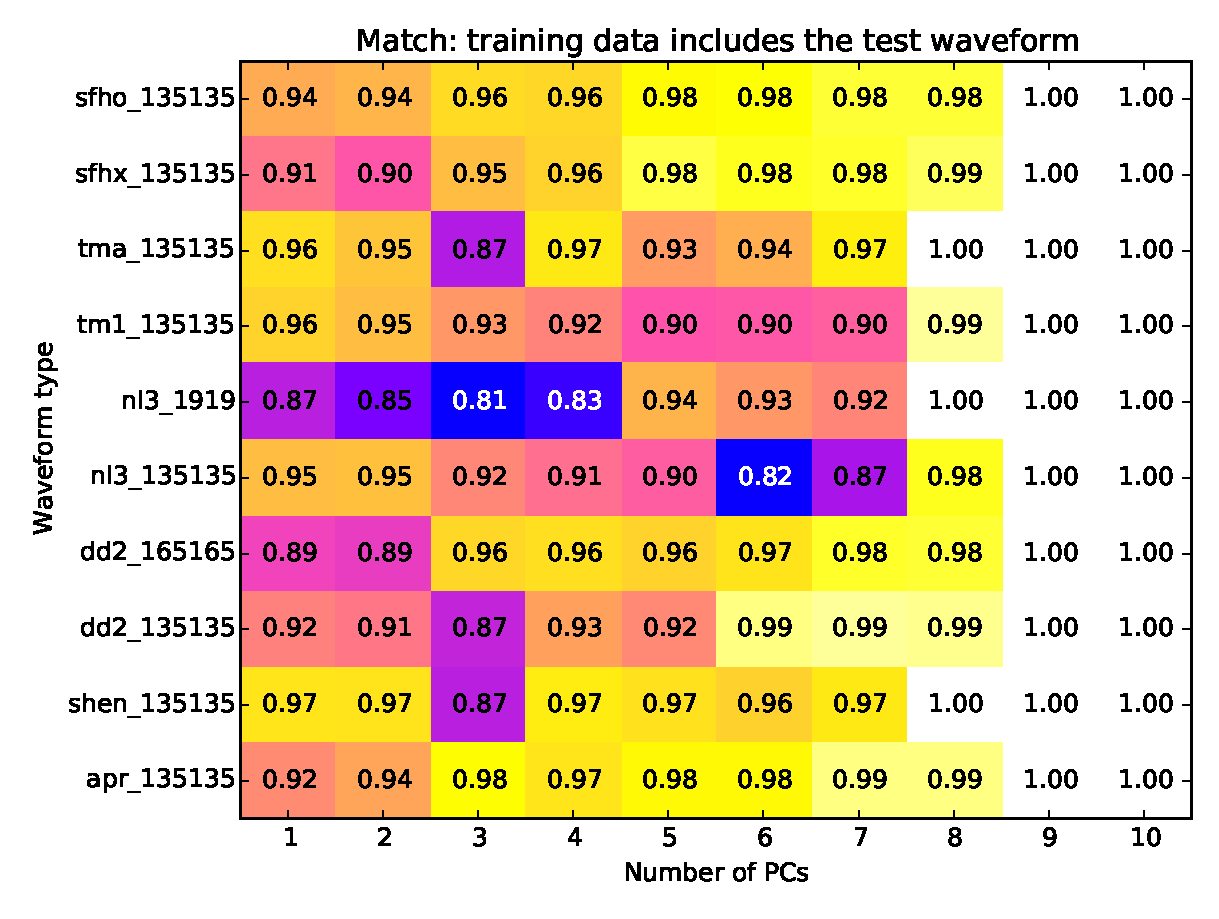
\includegraphics[width=\columnwidth]{figures/match_grid_inctestwav.pdf}
            \end{figure}
        \end{center}

\end{frame}

\begin{frame}
    \frametitle{Principal Component Analysis Of Short Bursts}

        \begin{center}
            \vspace{-0.5cm}
            \begin{figure}
                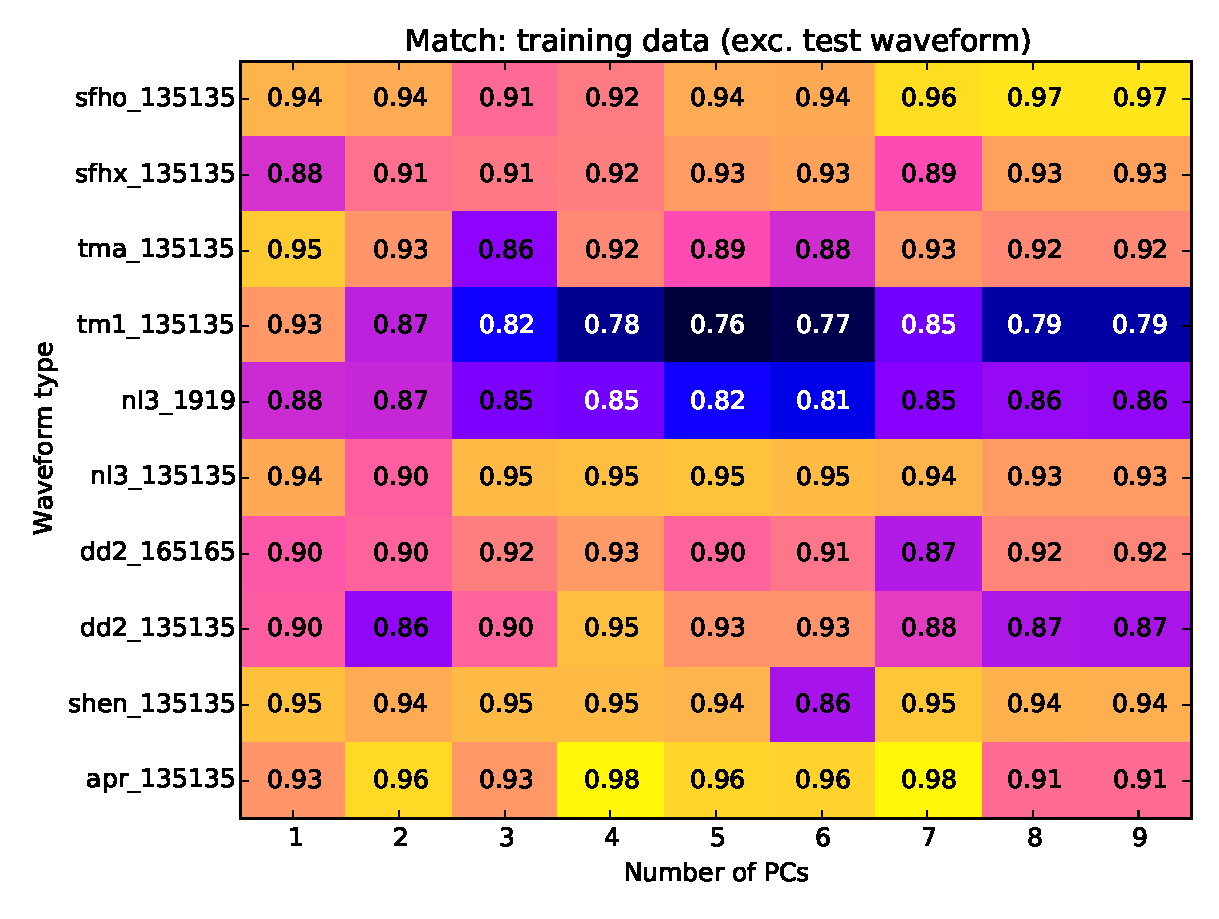
\includegraphics[width=\columnwidth]{figures/match_grid_exctestwav.pdf}
            \end{figure}
        \end{center}


\end{frame}

\end{document}

